\chapter{Additional work}
\label{cha:additional}

Two methods for structure initialization has been proposed (chapter \ref{cha:multi-view calibration}). However, a prior initialization for motion --rotation and translation-- is required. This chapter deals with a motion initialization, based on measurements and on the beforehand initialization.

This chapter is purely theoretical and experiments must be performed in order to get validation. Nevertheless, it is worth further research. Knowledge of \textit{linear algebra} and \textit{epipolar geometric} will be assumed. %On a first reading of this work, this chapter can be skipped.


\section{Preliminary}

% Even though knowledge of linear algebra and epipolar geometric is be assumed here,
Some preliminary concepts  of epipolar geometric are introduced as a reminder: essential matrix and camera resection.

\subsection{Essential matrix}
Now, consider a pair of camera matrices $P = [I | 0]$ and $P' = [R | t]$. The essential matrix has the form (see \cite[p257]{HZ2}):
\begin{equation}
E = [t]_{\times}R
\end{equation}
where
\begin{equation}
[t]_{\times} =
\begin{pmatrix}
      0    & -t_3  &  t_2 \\
      t_3  &  0    & -t_1 \\
     -t_2  &  t_1  &  0
\end{pmatrix},
\quad \quad \quad \quad \mbox{if~} t = (t_1, t_2, t_3)^T
\end{equation}


\subsection{Camera resection}
\label{sec:resection}

Extraction of cameras from the essential matrix is possible using SVD, more details can be found in \cite[p258-260, Result 9.19]{HZ2}. There are four possible solutions, except for overall scale, which
cannot be determined. Figure \ref{fig:resection} shows that a reconstructed point $X$ will be in front of both cameras in only one of these four solutions. Thus, testing a single point, to determine if it is in front of both cameras, is sufficient to decide between the solutions for the camera matrix~$P'$.

\begin{figure}[!htbp]
 \centering
 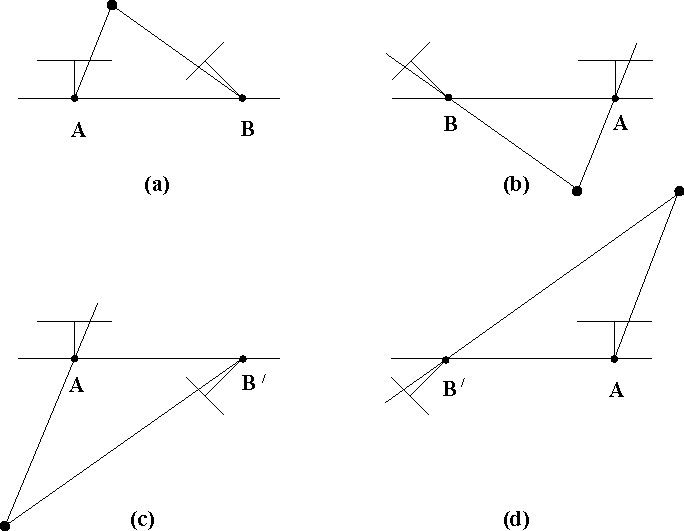
\includegraphics[width=0.6\textwidth]{images/resection.pdf}
 \caption{A reconstructed point $X$ is in front of both cameras only in (a).}
 \label{fig:resection}
\end{figure}
%



\section{Proposed method}

In this section, a proposed method is explained. This method is a generalization of camera resection (see section \ref{sec:resection}, or \cite[Result 9.19]{HZ2}). In \cite[p258, section 9.6.2]{HZ2} is stated that the overall scale cannot be determined,
% with resection the scale\footnote{Actually, the scale of the recovered translation} is unknown,
but it has been derived here that the scale is the norm of the original translation vector $\mathbf{t}$  (see theorem \ref{th:norm}). However, the norm of translation vector~$\mathbf{t}$ is usually unknown (recall that we want to recover the motion --$\mathbf{R}$ and $\mathbf{t}$-- from $\mathbf{E}$), but for theoretical purposes let's suppose for a moment it is known. \textbf{Note}: part of the following theorem proof is postponed until Appendix~\ref{ap:proof}.

% , it is possible to choose this scale in a more convenient way as explained in the following.

% \ref{th:norm}

% The demonstration will be left for later

% Then, a theorem must be proven first.

\subsection{Demonstration}
\begin{theorem}
\label{th:norm}
Suppose a given essential matrix $E=[\mathbf{t}]_{\times}R$, and the norm of $\mathbf{t}$ is known.
\[ \left.
  \begin{array}{l}
  E =[t]_{\times}R = S\,R \\
  ||t||=k
  \end{array} \right\}
  \Rightarrow
  \begin{array}{l}
  ~ ~ ~ \, E = U diag(k,k,0) V^T            \quad\quad\mbox{a SVD decomposition} \\
  ~ ~ ~ \, t= ~ ~ k\,u_3,  \quad\quad\quad\quad\quad\quad\quad u_3 \mbox{~last column of~} U \\
  \mbox{or~} t=-k\,u_3
  \end{array}
\]
\end{theorem}

\begin{proof}
\begin{align}
(\mbox{from theorem~} \ref{th:singular_values}, Appendix ~\ref{ap:proof})  & \quad\Rightarrow\quad E = U diag(k,k,0) V^T            \quad\quad\mbox{a SVD decomposition} \nonumber \\[3ex]
 t\,[t]_{\times} = 0 & \quad\Rightarrow\quad  t\,S = 0 \nonumber \\
                     & \quad\Rightarrow\quad  t \mbox{~is left null-space of~} S \nonumber \\
                     & \quad\Rightarrow\quad  t \mbox{~is left null-space of~} E, \quad \mbox{since~} E=SR \nonumber \\
                     & \quad\Rightarrow\quad  t = \alpha\,u_3, \quad\quad \alpha \in \mathbb{R}  \label{eq:alpha_u_3} \\
                     & ~~~~~~~~~~~~~~~~~~~~~~ \quad\quad u_3 \mbox{~last column of~} U  \nonumber \\
                     & ~~~~~~~~~~~~~~~~~~~~~~ \quad\quad ||u_3|| = 1  \label{eq:u_3_1}
\end{align}
We know that
\begin{align*}
 ||t||=k \overset{(\ref{eq:alpha_u_3})}{=} ||\alpha\,u_3|| = |\alpha|\,||u_3|| & \quad\overset{(\ref{eq:u_3_1})}{\Rightarrow}\quad  |\alpha| = k  \\
 & ~ \quad\Rightarrow\quad \alpha = k \mbox{~or~} \alpha = -k
\end{align*}
then
\begin{align*}
 t & = ~~||t||\,u_3 \mbox{~or~} \\
 t & = - ||t||\,u_3
\end{align*}
% \fbox{
%  \addtolength{\linewidth}{-2\fboxsep}%
%  \addtolength{\linewidth}{-2\fboxrule}%
%  \begin{minipage}{0.3\linewidth}
% \begin{align*}
%  t & = ~~||t||\,u_3 \mbox{~or~} \\
%  t & = - ||t||\,u_3
% \end{align*}
%  \end{minipage}
% }
\end{proof}


\subsection{Resection generalization}
% In order to complete the demonstration
% The previous theorem is needed to
The actual generalization is presented in the following theorem:
\begin{theorem}
\label{th:generalization}
For a given essential matrix $E = U diag(k,k,0) V^T$, where $||t||=k$, and first camera matrix
$P = [I | 0]$, there are four possible choices for the second camera matrix $P'$, namely
\begin{align*}
P' & = [~~UWV^T ~ ~| +k\,u3] \mbox{~or~} \\
   & = [~~UWV^T ~ ~| -k\,u3] \mbox{~or~} \\
   & = [~UW^TV^T ~ | +k\,u3] \mbox{~or~} \\
   & = [~UW^TV^T ~ | -k\,u3 ].
\end{align*}
where
\begin{equation}
\label{eq:W}
W =
\begin{pmatrix}
  0 & -1  & 0 \\
  1 &  0  & 0 \\
  0 &  0  & 1
\end{pmatrix}
\end{equation}
\end{theorem}

\begin{proof}
The proof is similar to \cite[Result 9.18 and Result 9.19]{HZ2}, the exception is the part where the translation is calculated, theorem \ref{th:norm} should be used. The full demonstration is left as an exercise for the reader\footnote{Please consider this as a revenge.}. \textbf{Notes}: \textbf{1.} four solutions are possible since there are two options for the rotation matrix and two for the translation: $t = ||t||\,u_3 \mbox{~or~} t=-||t||\,u_3$; \textbf{2.} as before, it is possible to determine the correct solution by testing with a single reconstructed point~$X$.
\end{proof}



\subsection{Scenario}

% The following assumption are considered valid in
Consider the following hypothetical scenario: \textbf{1.} only stereo pair will be taken into consideration instead of a multi-cameras setup; \textbf{2.} all cameras have the same $K$ intrinsic matrix, the identity: $K = I$; \textbf{3.} a \textbf{small} perturbation is the motion is produced by external causes, provoking a loss in the calibration. Figure \ref{fig:stereo} illustrates these assumptions:

\begin{figure}[!htbp]
 \centering
 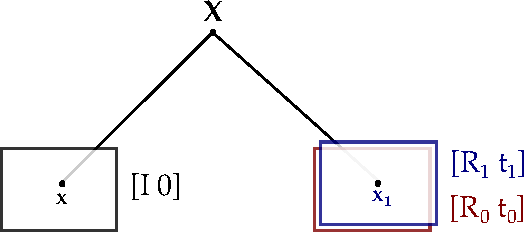
\includegraphics[width=0.4\textwidth]{images/stereo01.pdf}
 \caption{Stereo pair with and without perturbation.}
 \label{fig:stereo}
\end{figure}
where
\begin{itemize*}
 \item[-] {\color{red} $\mathbf{R_0}$, $\mathbf{t_0}$}: previous known motion (prior calibration or initialization).

 \item[-] {\color{blue} $\mathbf{R_1}$, $\mathbf{t_1}$}: new motion (unknown, but measurements in $[R_1~t_1]$ coordinate system.).
\end{itemize*}


\subsection{Application}
From the assumption number \textbf{3.} (small perturbations),
% can be rewritten for the translation as,
% \begin{equation}
% ||t_0 - t_1|| < \epsilon, \quad\quad\mbox{where~} \epsilon \mbox{ is ``small''}.
% \end{equation}
% The following notation will be used:
% \begin{equation}
%  t_0 \approx t_1
% \end{equation}
\begin{equation}
\label{eq:aprox}
 ||t_0|| \approx ||t_1||
\end{equation}

\noindent
Now, suppose that resection has been applied to the essential matrix $E$ obtained from the measurements between $[I~0]$ (left camera) and $[R_1~t_1]$. Then, from the correct solution, it is possible to obtain
\begin{equation}
 E \rightarrow R^*, t^*
\end{equation}

\noindent
For the exposed in \cite{HZ2} and % It has been shown that,
% Using
theorem \ref{th:generalization},
\begin{equation}
\left\{
  \begin{align}
  R_1 & = R^* \\
  t_1 & = ||t_1||\,t^*
  \end{align}
\right.
\end{equation}

\noindent
Then, using equation (\ref{eq:aprox}),
\begin{equation}
\label{eq:proposed_method}
\left\{
  \begin{align}
  R_1 & = R^* \\
  t_1 & \approx ||t_0||\,t^*
  \end{align}
\right.
\end{equation}

\noindent
And finally, the \textbf{proposed method} can be found in the last equation (\ref{eq:proposed_method}). In words can be summarized as: \textbf{1.} find essential matrix using the measurements; \textbf{2.} apply camera resection to recover motion, but with unknown scale factor in the translation; \textbf{3.} use the previous translation norm (our prior knowledge) to approximate the scale factor using theorem \ref{th:generalization}.

\subsection{Advantages / disadvantages}
\subsubsection{Advantages}
\begin{itemize*}
 \item Rotation matrix is can be calculated without ambiguities.
 \item Robust estimation for essential matrix exist; therefore, it can be robust to outliers.
\end{itemize*}

\subsubsection{Disadvantages}
\begin{itemize*}
 \item It is needed to calculated the essential matrix and then camera resection. It is more expensive computationally, in contrast with the use of the prior knowledge directly (i.e., previous motion: $[R_0~t_0]$).

 \item It has not been yet validate, see open questions below.
\end{itemize*}



\subsection{Open questions}

% Since experimentation have been centered in multi camera calibration, open questions are
As mentioned before, all the experimentation have been focused in multi camera calibration, and no time for this has been left. Therefore, there are still open questions, e.g.: 1. will it be possible to recover the scale factor of $||t1||$ with this method? 2. In that case, will it be better this initialization that the one already provided (i.e., previous motion)? Further research and experimentation is needed to validate the proposed method.







